\begin{figure}[tb]
\centering
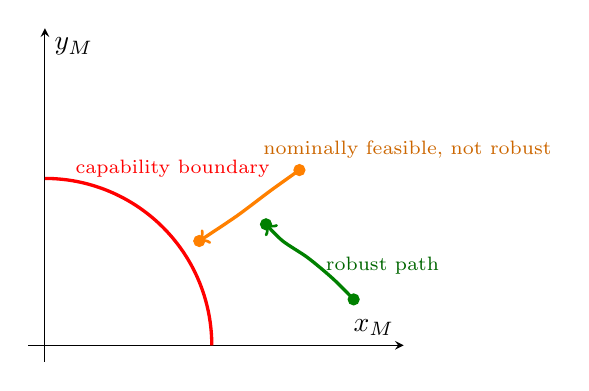
\begin{tikzpicture}
\begin{axis}[
 width=.72\linewidth,height=.48\linewidth,axis equal image,
 xmin=-.2,xmax=4.3,ymin=-.2,ymax=3.8,
 xlabel={$x_M$},ylabel={$y_M$},ticks=none,axis lines=middle,clip=false]
 \addplot[domain=0:90,samples=100,red,very thick] ({2*cos(x)},{2*sin(x)});
 \addplot[green!50!black,very thick,->,smooth]
  coordinates {(3.7,.55) (3.45,.8) (3.15,1.05) (2.85,1.25) (2.65,1.45)};
 \addplot[orange,very thick,->,smooth]
  coordinates {(3.05,2.1) (2.7,1.85) (2.3,1.55) (1.85,1.25)};
 \addplot[only marks,mark=*,green!50!black] coordinates {(3.7,.55) (2.65,1.45)};
 \addplot[only marks,mark=*,orange] coordinates {(3.05,2.1) (1.85,1.25)};
 \node[green!40!black,anchor=west,font=\scriptsize] at (axis cs:3.25,.95)
   {robust path};
 \node[orange!80!black,anchor=west,font=\scriptsize] at (axis cs:2.5,2.35)
   {nominally feasible, not robust};
 \node[red,anchor=south west,font=\scriptsize] at (axis cs:.25,1.9)
   {capability boundary};
\end{axis}
\end{tikzpicture}
\caption{Robust design is a path-containment requirement.  The green
temperature/saturation path remains feasible; the orange path crosses the
capability boundary although its nominal point is acceptable.}
\label{fig:robust-path}
\end{figure}

